\subsection*{Модель сегрегации Шеллинга в AnyLogic}
\addcontentsline{toc}{subsection}{Модель сегрегации Шеллинга в AnyLogic}

\textbf{Задание:}\\
Реализовать модель сегрегации Шеллинга в AnyLogic.\\

\textbf{Решение:}\\
Сначала была создана популяция размером -- 9000 агентов, заданная в дискретном пространстве и имеющую тип соседства -- Мурово. (Рисунок \ref{fig:scheling_anylogic1})
\begin{figure}[h]
	\centering 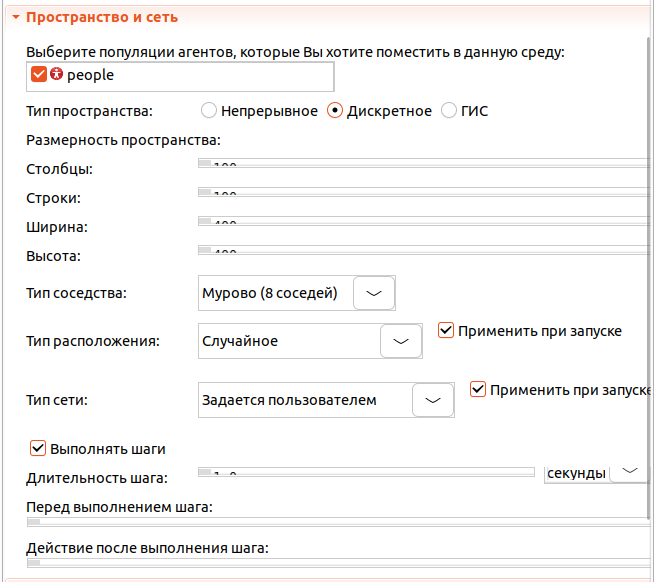
\includegraphics[scale=0.4]{scheling_anylogic1}
	\caption{Настройка популяции агентов}
	\label{fig:scheling_anylogic1}
\end{figure}

Цель данной модели заключается в том, чтобы промоделировать поведение людей. Существует несколько правил, по которым действую люди в данной модели:
\begin{enumerate}[topsep=0pt,itemsep=-1ex,partopsep=1ex,parsep=1ex]
	\item агент, который имеет только 1 агента соседа, переедет, если это сосед отличного цвета;
	\item агент, имеющих 2 соседей, не будет переезжать, если хотя бы один из них имеет тот же цвет, что и он сам;
	\item агент, проживающий по соседству от 3 до 5 человек, не будет переезжать, если хотя бы два из них будут цвета, что и он сам;
	\item агент с соседями от 6 до 8 человек не будет переезжать, если хотя бы 3 из них будут одного цвета.
\end{enumerate}

\newpage

Также стоит сказать, что изначально агентам задаются случайные цвета с равной вероятностью. Таким образом, агент будет иметь два параметра: цвет и состояние счастья, которое принимает тип boolean. (Рисунок \ref{fig:scheling_anylogic2})
\begin{figure}[h]
	\centering 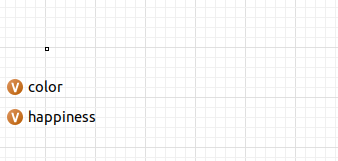
\includegraphics[scale=0.4]{scheling_anylogic2}
	\caption{Переменные и параметры агентов}
	\label{fig:scheling_anylogic2}
\end{figure}

Также в данной модификации модели рассматривается вариант при котором, агенты могут положительно взаимодействовать не только с соседями своего цвета, но и соседями других цветов. (Рисунок \ref{fig:scheling_anylogic3})
\begin{figure}[h]
	\centering 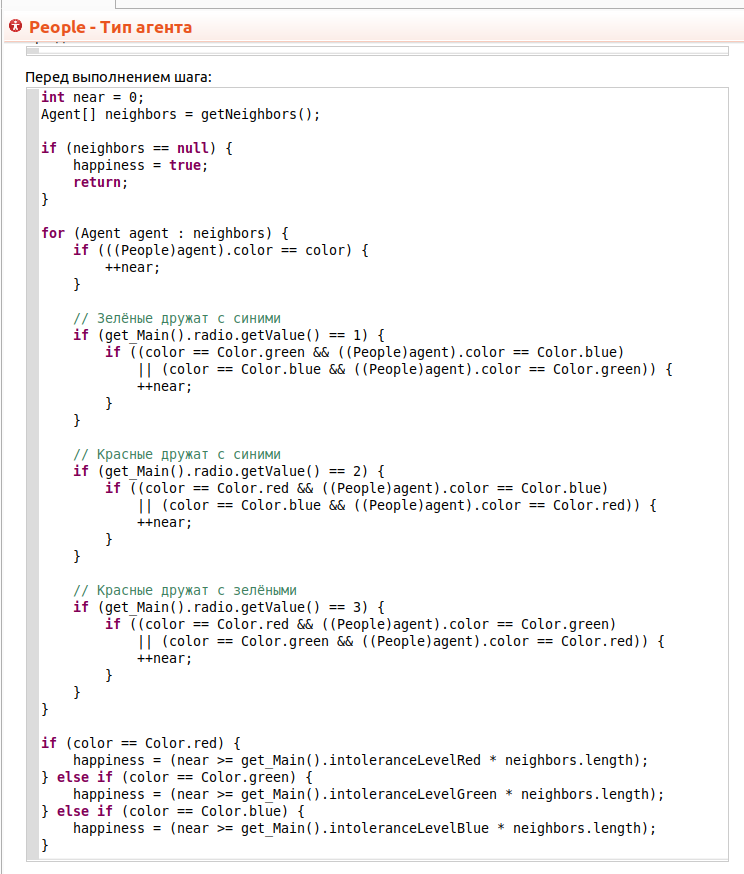
\includegraphics[scale=0.4]{scheling_anylogic3}
	\caption{Реализация алгоритма взаимодействия агентов}
	\label{fig:scheling_anylogic3}
\end{figure}

\newpage

Для сбора статистики кто среди агентов счастлив, а кто нет, была создана круговая диаграмма, которая отражает данные показатели. (Рисунок \ref{fig:scheling_anylogic4})
\begin{figure}[h]
	\centering 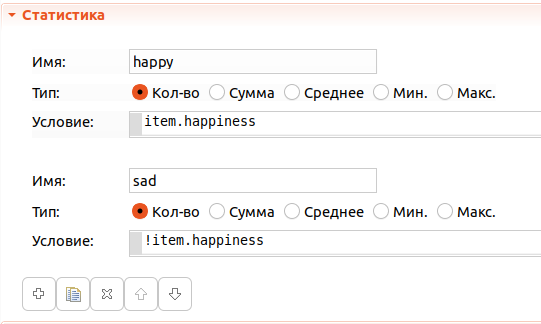
\includegraphics[scale=0.4]{scheling_anylogic4}
	\caption{Реализация алгоритма взаимодействия агентов}
	\label{fig:scheling_anylogic4}
\end{figure}

Также можно промоделировать различные сценарии взаимодействия агентов. (Рисунок \ref{fig:scheling_anylogic5})
\begin{figure}[h]
	\centering 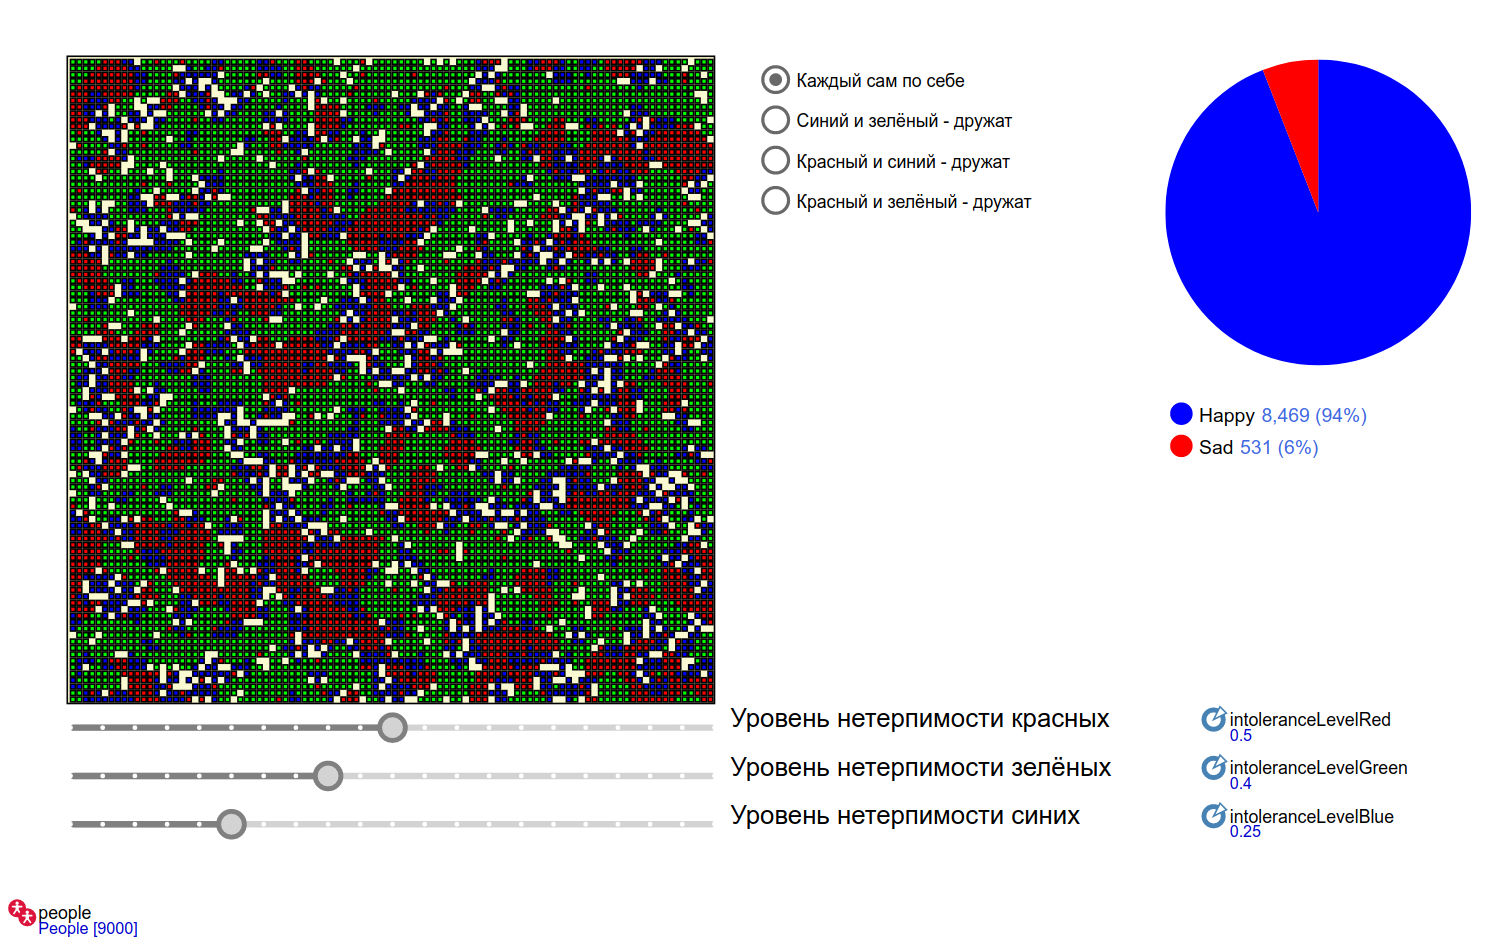
\includegraphics[scale=0.3]{scheling_anylogic5}
	\caption{Результат работы модели}
	\label{fig:scheling_anylogic5}
\end{figure}

Таким образом, была реализована модель сегрегации Шеллинга при различных условиях взаимодействия агентов.